% =========================================================================
% ESWA 论文中文版(article + ctex 单栏中文排版,非毕设 ctexart 体例)
% 编译:xelatex eswa_zh; bibtex eswa_zh; xelatex eswa_zh; xelatex eswa_zh
% =========================================================================
\documentclass[11pt,a4paper]{article}
\usepackage[UTF8]{ctex}
\usepackage[margin=1in]{geometry}
\usepackage{microtype}
\usepackage{graphicx}
\usepackage{booktabs}
\usepackage{amsmath,amssymb}
\usepackage{array}
\usepackage{makecell}
\usepackage{multirow}
\usepackage{xcolor}
\usepackage{enumitem}
\usepackage[numbers]{natbib}
\usepackage[hidelinks]{hyperref}
\usepackage{pifont}
\usepackage{tikz}
\usetikzlibrary{positioning,arrows.meta,fit,backgrounds,shapes.geometric}
\usepackage{xurl}
\sloppy
\renewcommand{\arraystretch}{1.15}
\newcommand{\qtype}[1]{\texttt{\small #1}}
\newcommand{\op}[1]{\textsc{\small #1}}

\title{\bfseries 面向雷达电子战情报分析的\\策略路由式可审计决策支持系统}
\author{作者姓名\\ \small 单位,中国}
\date{}

\begin{document}
\maketitle

\begin{abstract}
\noindent
雷达电子战(EW)情报分析员需要在碎片化的威胁数据上回答复杂问题——枚举某平台搭载的全部辐射源、对多个工作约束求交集、确认某项能力\emph{不存在},或针对敌方防空雷达给出对抗建议。在这些场景中,不完整或错误的回答会带来作战代价,且分析员必须能把每一条结论\emph{追溯到来源}。本文提出一个面向雷达电子战情报分析的智能决策支持系统,构建于一个经策展的雷达知识图谱之上(RadarKG-v2;4\,827 个实体、16\,513 条三元组)。其检索引擎摒弃了当前 GraphRAG 所依赖的 top-$K$ 范式:我们指出 top-$K$ 隐含了一个关于\emph{答案几何}的假设,该假设在枚举、求交与求补类查询上系统性失效;我们以一套由六个\emph{类型化检索算子}构成的算子族取而代之,每个算子均由某一查询类的信息需求推导而来,并由一个轻量大语言模型(LLM)分发器选择。一个\emph{规划—执行—校验}智能体负责分解多步分析请求,同时使大语言模型\emph{不进入信任路径}:每个事实与数字都由确定性的知识图谱算子产生,并附带其来源与置信度。一个以条令为根基的模块,通过加权集合覆盖式推演,把敌方战斗序列转化为可审计的对抗建议。在公开发布的 499 题双语基准上,系统达到 \textbf{88.6\%} 的准确率,而强基线为 52.7\%(提升 $+35.9$ 个百分点),单次查询成本仅 \textbf{\$0.00041};其问题类型学还可零重训迁移到通用领域知识图谱。
\end{abstract}

\noindent\textbf{关键词:} 智能决策支持系统;电子战情报;知识图谱问答;检索增强生成;可审计大语言模型系统

% =========================================================================
\section{引言}
\label{sec:intro}

\paragraph{作战层面的决策。}
雷达电子战(EW)情报分析员支撑着一个反复出现的决策:给定一批碎片化、多来源的威胁数据,刻画某个辐射源或平台,并最终给出对其作战的建议。驱动该决策的问题极少是单一事实,而往往是:某型系统\emph{配备了哪些}防空雷达、某平台在某频段\emph{有多少}个辐射源、某威胁雷达\emph{是否}具备已知的对干扰寻的(home-on-jam)能力,或\emph{用什么}对抗手段能击败某型敌方雷达、剩余风险几何。在作战场景中,一次\emph{不完整}的枚举(漏掉一个辐射源)或一次\emph{错误}的"安全"判断(把实际存在的能力误报为不存在)都不是排序误差——它有代价。由此引出两条现成问答工具无法满足的要求:对所提问题的类别而言,答案必须\emph{完整且结构正确};并且每条结论都必须可\emph{追溯}到具名来源,使分析员能判断其可信程度。

\paragraph{为何通用 GraphRAG 在此不胜任。}
知识图谱检索增强生成(GraphRAG)\citep{edge2024graphrag,gutierrez2024hipporag,peng2025graphrag} 已成为将大语言模型(LLM)接地于结构化领域知识的标准做法。然而几乎所有 GraphRAG 变体——社区摘要、个性化 PageRank、LLM 路径模板、束搜索 \citep{luo2024rog,sun2024tog,ma2025tog2}——检索的都是一个按表面相关性排序的 top-$K$ 段落或三元组集合。top-$K$ 默默假设答案是一个\emph{可按相关性排序的小集合}。对于分析员最棘手的问题,这一假设恰恰错误:穷举计数受 $K$ 上界约束,而答案集合并不受其约束;多约束筛选无法用排序表达;非成员性断言无法靠检索"已有事实"来确认。这种失效是\emph{信息论意义}上的,而非模型能力弱或 $K$ 取得太小所致(我们将证明,把检索预算从 $K{=}8$ 增至 $K{=}20$ 仅带来 $+2.4$ 个百分点的提升)。因此,面向该领域的决策支持系统需要一个其\emph{访问模式与问题答案几何相匹配}的检索层,外加一个分析员可审计的编排层。

\paragraph{贡献。}
我们设计、实现并评估了一个面向雷达电子战情报分析的智能决策支持系统。按分析员接触它们的顺序,其贡献为:
\begin{enumerate}[leftmargin=1.4em,itemsep=2pt]
\item 一个\textbf{领域知识库}(RadarKG-v2)及一个已部署的问答前端,分析员可用自然语言(中文或英文)查询;
\item 一个\textbf{策略路由式检索引擎},以六个类型化算子组成的算子族取代 top-$K$,每个算子均由某一查询类的信息需求推导而来。这是系统的分析内核;在公开基准上,它把端到端准确率从 52.7\% 提升到 88.6\%;
\item 一个\textbf{规划—执行—校验智能体},分解多步请求,并且关键地使 LLM \emph{不进入信任路径}:所有事实与数字均来自确定性图算子,并附来源与置信度层级,因此输出是一份\emph{可审计的情报报告},而非自由生成的文本;
\item 一个\textbf{电子战对抗决策支持模块},通过加权集合覆盖式推演,把敌方战斗序列转化为以条令为根基的对抗建议,且每条建议均带溯源;
\item 一个\textbf{公开发布的双语基准}(RadarKG-QA-499)及一份诚实的运行成本刻画(单次查询 \$0.00041),使系统主张可复现、可部署性被量化。
\end{enumerate}

% =========================================================================
\section{系统概览与分析员的决策流水线}
\label{sec:overview}

图~\ref{fig:decision} 从分析员视角展示了系统。一条自然语言请求进入\emph{规划器},由其判断这是单次查询还是多步任务。每个查询由一个轻量\emph{分发器}路由到其访问模式与之匹配的类型化检索算子,算子\emph{仅对知识图谱}执行。结果送入\emph{校验器},检查是否为空或可疑输出,并可触发一轮重规划(例如对图谱尚未覆盖的型号做一次联网查询)。分析员收到的报告中,每一行都带其来源与置信度;基于同一证据,电子战模块可产出对抗建议。LLM 仅以分发器、规划器和最终\emph{措辞}阶段的身份出现——绝不充当事实或数字的来源。

\begin{figure*}[t]
\centering
\resizebox{\linewidth}{!}{%
\begin{tikzpicture}[
  font=\small,
  node distance=7mm and 10mm,
  box/.style={draw,rounded corners,align=center,inner sep=4pt,minimum height=9mm},
  kg/.style={draw,cylinder,shape border rotate=90,aspect=0.25,align=center,inner sep=3pt},
  >={Stealth[]}]
\node[box,fill=blue!6] (q) {分析员请求\\\scriptsize(自然语言,中/英)};
\node[box,right=of q,fill=blue!6] (plan) {规划器\\\scriptsize 任务分解\\\scriptsize +校验/重规划};
\node[box,right=of plan] (disp) {分发器\\\scriptsize 答案几何\\\scriptsize $\to$ 算子};
\node[box,right=of disp,fill=green!8] (ops) {类型化算子\\\scriptsize lookup / exhaustive /\\\scriptsize complement / path /\\\scriptsize join / dual-subgraph};
\node[kg,below=11mm of ops,fill=orange!12] (kg) {雷达\\KG\\\scriptsize 1.65万};
\node[box,right=of ops,fill=yellow!15] (rep) {可审计报告\\\scriptsize 每行:\\\scriptsize 来源+置信度};
\node[box,below=11mm of rep,fill=red!8] (ew) {电子战对抗建议\\\scriptsize 集合覆盖推演};
\draw[->] (q)--(plan); \draw[->] (plan)--(disp); \draw[->] (disp)--(ops);
\draw[->] (ops)--(kg); \draw[->] (ops)--(rep); \draw[->] (rep)--(ew);
\draw[->] (rep.south) to[bend right=18] node[midway,below,font=\scriptsize]{缺口} (plan.south);
\begin{scope}[on background layer]
\node[draw,dashed,rounded corners,fit=(disp)(ops)(kg),inner sep=7pt,
  label=below:{\scriptsize\itshape 事实与数字:确定性产生,LLM 不进入信任路径}]{};
\end{scope}
\end{tikzpicture}%
}
\caption{分析员的决策流水线。语言模型仅充当规划器、分发器与最终措辞;每个事实、计数与"不存在"断言均由确定性知识图谱算子产生并附带溯源。内部各阶段视图见图~\ref{fig:pipeline}。}
\label{fig:decision}
\end{figure*}

% =========================================================================
\section{知识库}
\label{sec:kg}

RadarKG-v2 含 4\,827 个实体、12\,219 条实体间关系边,外加约 80 种类型化数值/类别属性(共 16\,513 条三元组),由一部 472 页的机载雷达手册(全文 OCR)、Wikidata 的 SPARQL 拉取以及 Wikipedia 摘要构建而成。原产国与研制方的覆盖率分别为 93.4\% 与 87.0\%。模式(schema)为英文,而取值词表为中英混合,这反映了工业级国防知识图谱的真实填充方式。每条三元组都携带 \texttt{source}(来源)、\texttt{confidence}(置信度)与 \texttt{evidence}(证据指针);正是这些元数据使系统能为每一行答案附上溯源(见 \S\ref{sec:agent})。数值属性命名为 \texttt{<属性>\_<单位>}(如 \texttt{range\_km}、\texttt{peak\_power\_kW});任一单项数值属性的覆盖率都是部分的(约占实体的 20\%--25\%),因此聚合类答案始终报告样本规模 $N/M$,而不暗示其完整性。

% =========================================================================
\section{检索引擎:让访问模式匹配答案几何}
\label{sec:engine}

\subsection{答案几何失配}
top-$K$ 检索擅长\emph{点查询},却在\emph{聚合查询}上结构性地错误——这与数据库在 OLTP 的 B 树索引和 OLAP 的扫描之间所作的区分如出一辙 \citep{codd1970relational}。威胁知识图谱中常见的三类查询模式,各因不同且可计算的原因击穿 top-$K$:\textbf{无界枚举}(答案集合可超过任意 $K$)、\textbf{多约束求交}(排序无法表达逻辑"与")、\textbf{求补/非成员}(知识图谱只存正事实,故"不存在"是非局部的)。我们称之为\emph{答案几何失配}:检索原语的输出形状与问题所需答案的形状不匹配。

\subsection{一套推导而非拼凑出来的类型化算子}
我们不逐一为失败打补丁,而是枚举 top-$K$ 无法满足的信息需求类别,为每一类推导一个算子,并为 top-$K$ \emph{确能}满足的那一类补上 \op{lookup}(表~\ref{tab:reqs})。每个算子都是满足其所在行信息需求的\emph{最小}访问模式。十一种面向分析员的问题类型确定性地映射到这六个算子(表~\ref{tab:typology})。一个零样本 LLM 分发器(路由准确率 93.0\%)读取问题并选择算子;一个贯穿全局的\textbf{双语别名层}(五级级联:直接匹配 $\to$ 614 形态别名索引 $\to$ 频段归一 $\to$ 后缀剥离 $\to$ 等价类合并)化解使朴素图查询失败的中英混合取值。图~\ref{fig:pipeline} 展示了内部各阶段。

\begin{table*}[t]
\centering\small
\caption{算子族的信息需求推导。每一行依据满足其需求的最小访问模式确定其算子;top-$K$ 在每一行因不同原因失效。}
\label{tab:reqs}
\setlength{\tabcolsep}{4pt}
\begin{tabular}{p{0.16\linewidth} p{0.27\linewidth} p{0.28\linewidth} p{0.20\linewidth}}
\toprule
\textbf{模式} & \textbf{信息需求(最小)} & \textbf{为何 top-$K$ 失效} & \textbf{推导出的算子} \\
\midrule
身份/事实型     & 单条最佳匹配三元组                       & (无——top-$K$ 即可满足)                       & \op{lookup} = BM25 $\oplus$ 向量 $\oplus$ RRF \\
无界枚举        & 某关系的\emph{完整}头/尾集合             & $K$ 是上界,而答案集合不是                     & \op{exhaustive} = $\{h \mid (h,r,t)\!\in\!\text{KG}\}$ \\
多约束"与"      & $N$ 个关系头集合的交集                    & 排序无法表达"与",会混淆信号                   & \op{constrained-join} = $\bigcap_i \text{heads}(r_i,t_i)$ \\
求补/不存在     & 完整的\emph{已知}集合,再显式给出缺口      & 知识图谱只存正事实,"不存在"是非局部的         & \op{complement} = 先枚举再核验 \\
组合 $(k\!\geq\!2)$ & 跨 $k$ 个关系、保留跳数结构的路径    & top-$K$ 是扁平的,会丢失跳边界                 & \op{path-plan} = $\text{tails}_{r_1}\!\circ\!\dots\!\circ\!\text{tails}_{r_k}$ \\
二元比较        & \emph{双方}子图均显式且对齐              & top-$K$ 可能饿死一方,且无法对齐               & \op{dual-subgraph} = 并行 $\text{tails}(A,B)$ + 集合运算 \\
\bottomrule
\end{tabular}
\end{table*}

\begin{table}[h]
\centering\small
\caption{分析员问题类型 $\to$ 算子(11 类类型学)。}
\label{tab:typology}
\begin{tabular}{p{0.35\linewidth} p{0.27\linewidth} l}
\toprule
\textbf{类型} & \textbf{信号} & \textbf{算子} \\
\midrule
\qtype{single\_hop}                                                 & 实体+属性     & \op{lookup} \\
\qtype{relation\_inverse,} \qtype{agg\_count,} \qtype{agg\_enum}    & 无界枚举      & \op{exhaustive} \\
\qtype{two\_hop\_bridge,} \qtype{three\_hop\_chain}                 & 组合 $k\!\geq\!2$ & \op{path-plan} \\
\qtype{attr\_filter}                                                & 约束之"与"    & \op{constrained-join} \\
\qtype{negation,} \qtype{unanswerable}                              & 不存在        & \op{complement} \\
\qtype{set\_compare}                                                & 两实体        & \op{dual-subgraph} \\
\qtype{distractor}                                                  & 消歧          & \op{lookup} \\
\bottomrule
\end{tabular}
\end{table}

\begin{figure}[h]
\centering
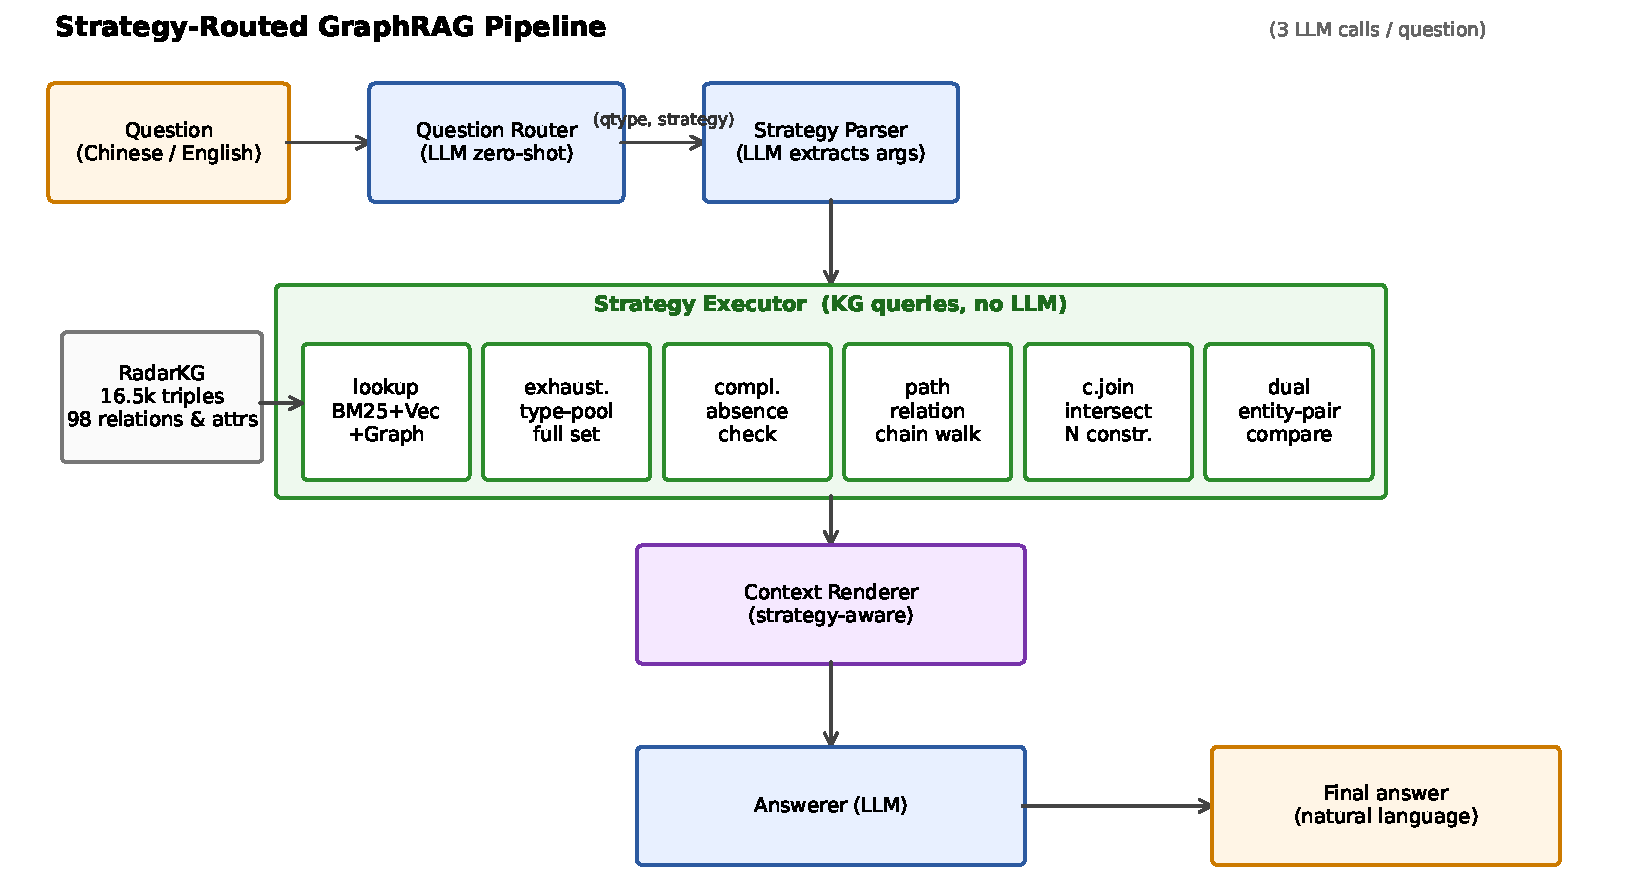
\includegraphics[width=0.95\linewidth]{figures/fig1_pipeline.pdf}
\caption{检索引擎的内部各阶段:LLM 分发器/解析器/作答器,外加一个仅查图谱的执行器。知识图谱只在执行器中被查询。}
\label{fig:pipeline}
\end{figure}

% =========================================================================
\section{智能体编排与可审计性}
\label{sec:agent}

单次查询很少能对应分析员的真实请求(如"列出该平台的防空雷达\emph{并}分别给出对抗建议")。一个规划—执行—校验智能体处理此类任务。(i) 一个\emph{规划器} LLM 把请求分解为带显式\emph{数据流}的步骤列表:某步参数可引用前一步的结果($\$s_N$),而 \texttt{foreach}\,$\$s_N$ 对前一步结果集合中的每一项施加某工具。(ii) 各步骤\emph{确定性}执行;实体集合在步骤间以值传递,绝不由 LLM 二次转写,因此不发生漂移。(iii) 一个\emph{校验器}检查执行轨迹中的确定性缺口信号(空集、"未收录"、工具出错、\texttt{foreach} 为空);遇缺口则产出一份修订计划(仅一次)——通常是为超出覆盖的型号添加一次联网查询,或放宽某项约束——并重跑。

\paragraph{LLM 不进入信任路径。}
这是本系统面向决策支持场景的核心设计原则。输出中的每个事实、计数与"不存在"断言均由对知识图谱的确定性算子产生;LLM 仅\emph{路由}、\emph{规划}与\emph{措辞}。情报报告为每条结论附上产生它的三元组的 \texttt{source} 与 \texttt{confidence},并且智能体逐字附上确定性产物,而不让 LLM 重新复述——我们观察到,自由生成的最终文本会臆造图谱中并不存在的参数。因此可审计性是一种结构性属性,而非一句提示词指令。

% =========================================================================
\section{电子战对抗决策支持}
\label{sec:ew}

同样的溯源纪律驱动着系统价值最高的输出:针对敌方辐射源的对抗建议。一个\emph{条令本体}编码了干扰技术与电子反对抗(ECCM)技术,以及一个介于 ECCM 技术集 $E$ 与干扰技术集 $J$ 之间的\emph{击败}关系 $\mathcal{D}\subseteq E\times J$,均由开源电子战条令策展而来 \citep{adamy2001ew101,schleher1999ew,zhang2023cognitiveew}。给定一部威胁雷达,推荐器对每项技术返回三分判定——\emph{可行}、\emph{被抵消}(该雷达配备了能击败它的 ECCM)或\emph{应避免}——每项均标注条令来源与置信度层级(关键词匹配 / LLM 引文核验 / 条令先验)。

对于多辐射源的敌方战斗序列,系统把对抗手段选择形式化为一个\textbf{加权集合覆盖}问题:选取一个最小权重的干扰技术集合以覆盖全部威胁辐射源,采用经典的 $H_n\!\approx\!\ln n + 1$ 近似保证以贪心法求解 \citep{chvatal1979setcover}。输出是一份可审计的推演方案:哪项技术覆盖哪些威胁、剩余未覆盖集合,以及每个选择的条令依据。这是严格意义上的决策支持功能 \citep{power2002dss}——它为人类分析员组织并论证一个选择,而决策权仍由分析员保留。条令本体含 17 项干扰技术、16 项 ECCM 技术与 14 条推荐规则;其保真性与溯源性在 \S\ref{sec:eval-ew} 评估。

% =========================================================================
\section{评估}
\label{sec:eval}

\paragraph{设置。} 所有系统均使用 DeepSeek-Chat \citep{deepseekv3_2024}。我们在全部 499 道基准题上比较三个系统:\textbf{基线} = BM25 \citep{robertson2009bm25} + 双编码器 \citep{xiao2024bge} + 倒数排名融合 \citep{cormack2009rrf} + 2 跳扩展,top-$K{=}8$;一个\textbf{零样本路径规划器}(受 RoG 启发 \citep{luo2024rog},单策略检索);以及我们的 \textbf{Strategy} 引擎。置信区间为配对自助法(1000 次重采样)。所选对照集刻意做强:路径规划基线即 Reasoning-on-Graphs(RoG)\citep{luo2024rog}——一种最新的推理路径式 GraphRAG 方法,既以零样本评估,又作为\emph{有监督上界}在两个 7B 底座(含 RoG 原始底座)上忠实 LoRA 微调(见 \S\ref{sec:related});Adaptive-RAG \citep{jeong2024adaptiverag} 与 ByoKG-RAG \citep{byokgrag2025} 等近期路由/工具方法在\emph{种类}上不同(它们改变检索深度或来源,而非检索原语的语义),详见 \S\ref{sec:related}。

\subsection{基准及其必要性}
RadarKG-QA-499 含 499 道自动生成、可机器验证的题目,按 11 类分层,另加一个 26 题的分布外(OOD)双语压力子集,把英文/缩写别名替入中文模板。我们之所以发布它,是因为\emph{没有}公开 KGQA 基准对高基数答案集合做分层——而后者正是检索预算结构性失效最清晰的信号:RadarKG-QA-499 的计数题中位基数是次接近公开基准(KQA Pro)的 $3.4$ 倍、高基数占比是其 $3$ 倍,且多约束与三跳问题上存在同样的差距(图~\ref{fig:cardinality})。金标答案直接取自知识图谱的真值内容(完整关系集合、真实交集、$k$ 跳终点集合),\emph{独立于任何受测系统};三个系统都去逼近同一目标,故比较公平且非循环——top-$K$ \emph{原则上}可返回完整集合,但受 $K$ 结构性约束而做不到,这正是所研究的现象(连我们的算子在计数题上也未达 100\%,这说明该指标并非读一遍图谱即可平凡满足)。判对标准是精确匹配(计数等于金标计数、集合等于金标集合),故该指标度量的是\emph{对 KG 的忠实度}:残余 KG 噪声同时存在于金标与任何忠实系统的输出中,因而限制绝对准确率但不影响比较的公平性。\op{constrained-join} 的等价类回退(合并相关的 \texttt{countryOfOrigin}/\texttt{operatedBy} 关系)被设为仅在严格交集为空时触发,且金标用严格关系算出;它仅在 50 道多约束题中的 2 道上触发、使其准确率改变 $0.0$ 个百分点,故多约束增益并非关系放宽的产物。

\begin{figure}[h]
\centering
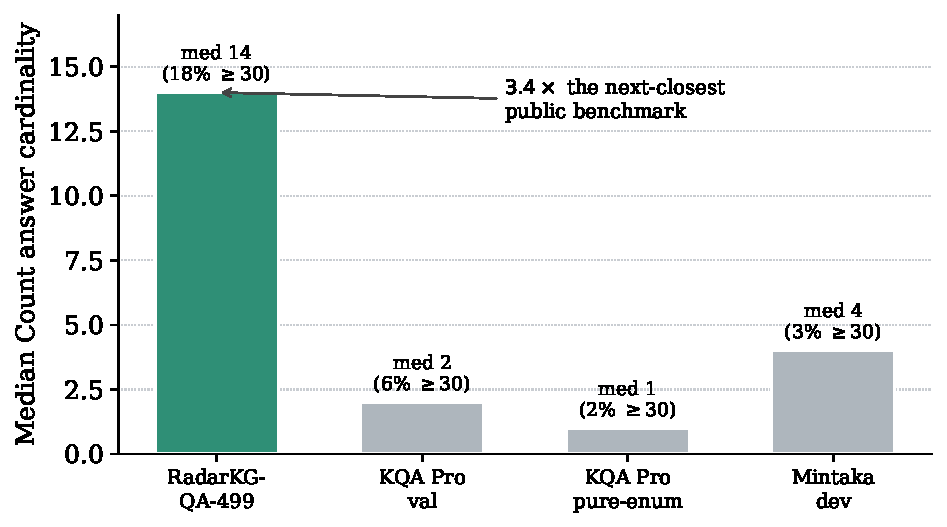
\includegraphics[width=0.82\linewidth]{figures/fig4_cardinality.pdf}
\caption{各基准计数题的答案基数。RadarKG-QA-499 的中位基数是次接近公开基准的 $3.4$ 倍、高基数($\geq\!30$)占比是其 $3$ 倍——这正是分析员的枚举类问题真实所处的区间。}
\label{fig:cardinality}
\end{figure}

\subsection{决策质量结果}
Strategy 引擎总体达 \textbf{88.6\%},而基线为 52.7\%、路径规划器为 60.3\%:分别提升 $+35.9$ 与 $+28.3$ 个百分点,配对置信区间严格为正,并在 11 类中的 9 类胜出(表~\ref{tab:main}、图~\ref{fig:results})。增益恰好集中于分析员最易出错之处:计数辐射源 $+58$ 个百分点、多约束筛选 $+80$ 个百分点、三跳链 $+70$ 个百分点。增加检索预算无法替代:$K{=}8\!\to\!20$ 的基线仅提升 $+2.4$ 个百分点,而 Strategy 仍以 $+33.5$ 个百分点领先 $K{=}20$ 基线——因为没有任何 $K$ 能为结构上大于 $K$ 的答案集合设界。

\begin{table*}[t]
\centering\small
\caption{RadarKG-QA-499 上的决策质量($n{=}499$,准确率 \%,含 95\% 配对自助置信区间)。Strategy 在 11 类中的 9 类以严格为正的区间胜出。}
\label{tab:main}
\setlength{\tabcolsep}{3.5pt}
\begin{tabular}{l r l l l l l}
\toprule
\textbf{类型} & \textbf{n} & \textbf{基线} & \textbf{RoG} & \textbf{Strategy} & \textbf{$\Delta$ S$-$B} & \textbf{$\Delta$ S$-$RoG} \\
\midrule
\qtype{agg\_count}        & 50 & 4.0 [0, 10] & 38.0 [26, 50] & \textbf{62.0 [48, 74]} & $+$58 [$+$44, $+$72] & $+$24 [$+$12, $+$36] \\
\qtype{agg\_enum}         & 50 & 46.0 [32, 58] & 92.0 [84, 98] & \textbf{96.0 [90, 100]} & $+$50 [$+$36, $+$64] & $+$4 [$+$0, $+$10] \\
\qtype{attr\_filter}      & 50 & 12.0 [4, 22]  & 0.0           & \textbf{92.0 [84, 98]} & $+$80 [$+$66, $+$92] & $+$92 [$+$84, $+$98] \\
\qtype{relation\_inverse} & 50 & 40.0 [26, 54] & 74.0 [62, 86] & \textbf{86.0 [76, 94]} & $+$46 [$+$32, $+$60] & $+$12 [$+$4, $+$22] \\
\qtype{three\_hop\_chain} & 30 & 23.3 [10, 40] & 50.0 [33, 70] & \textbf{93.3 [83, 100]} & $+$70 [$+$53, $+$87] & $+$43 [$+$23, $+$63] \\
\qtype{two\_hop\_bridge}  & 80 & 40.0 [29, 51] & \textbf{95.0 [90, 99]} & 88.8 [81, 95] & $+$49 [$+$38, $+$60] & $-$6 [$-$14, $+$0] \\
\qtype{single\_hop}       & 80 & 83.8 [75, 91] & 11.2 [5, 19]  & \textbf{86.2 [79, 94]} & $+$2.5 [$+$0, $+$6] & $+$75 [$+$65, $+$85] \\
\qtype{set\_compare}      & 40 & 97.5 [93, 100] & 85.0 [73, 95] & 97.5 [93, 100] & 0 & $+$13 [$+$3, $+$23] \\
\qtype{negation}          & 40 & 100.0          & 97.5 [93, 100] & 100.0 & 0 & $+$3 [$+$0, $+$8] \\
\qtype{unanswerable}      & 20 & 90.0 [75, 100] & \textbf{100.0} & 90.0 [75, 100] & 0 & $-$10 [$-$25, $+$0] \\
\qtype{distractor}        & 9  & 100.0          & 66.7 [33, 100] & 100.0 & 0 & $+$33 [$+$0, $+$67] \\
\midrule
\textbf{总体} & \textbf{499} & \textbf{52.7 [48, 57]} & \textbf{60.3 [56, 65]} & \textbf{88.6 [86, 91]} & \textbf{$+$35.9 [$+$32, $+$40]} & \textbf{$+$28.3 [$+$24, $+$33]} \\
\bottomrule
\end{tabular}
\end{table*}

\begin{figure}[h]
\centering
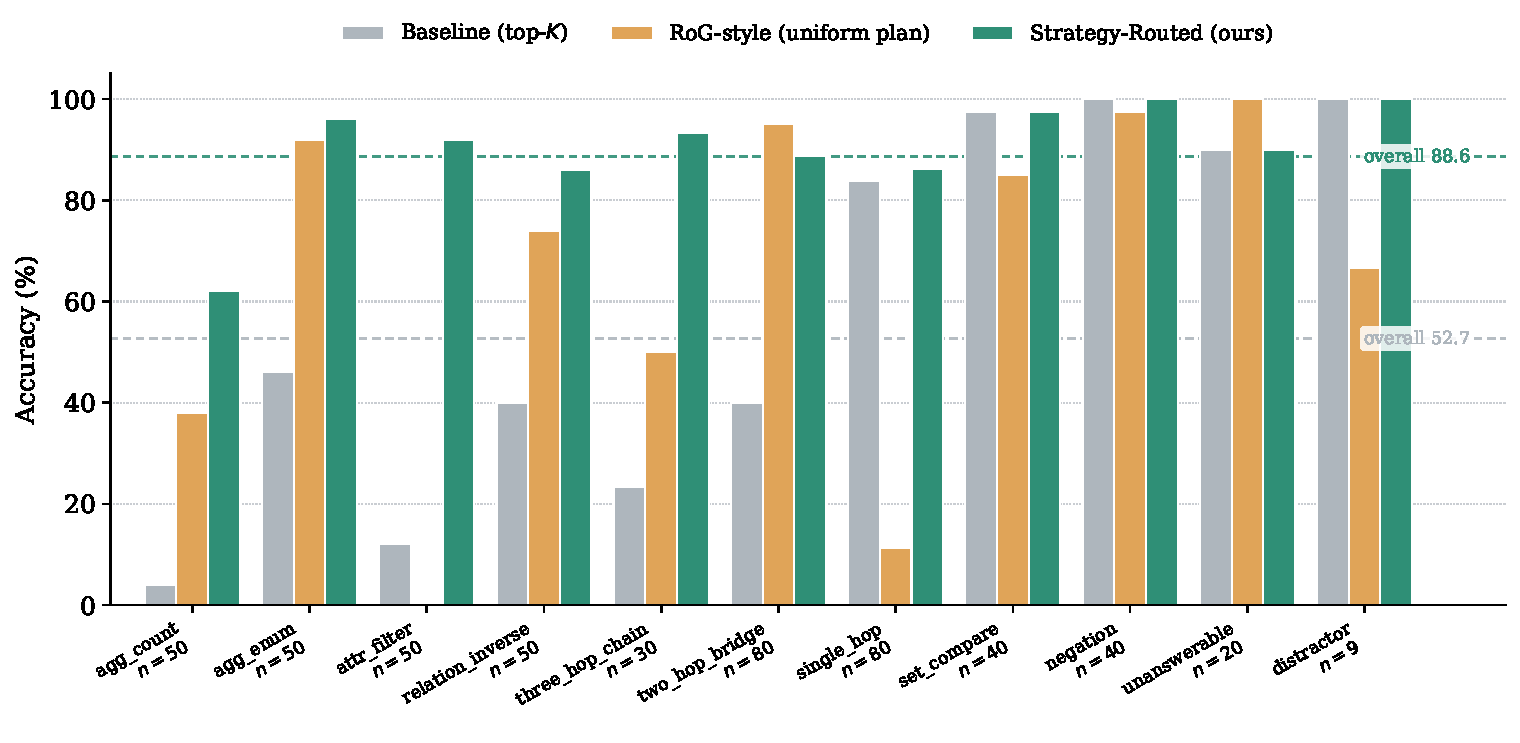
\includegraphics[width=0.98\linewidth]{figures/fig2_main_results.pdf}
\caption{分类别准确率:基线 vs 路径规划器 vs Strategy。增益集中于高答案几何类型(计数、筛选、多跳)。}
\label{fig:results}
\end{figure}

\begin{figure}[h]
\centering
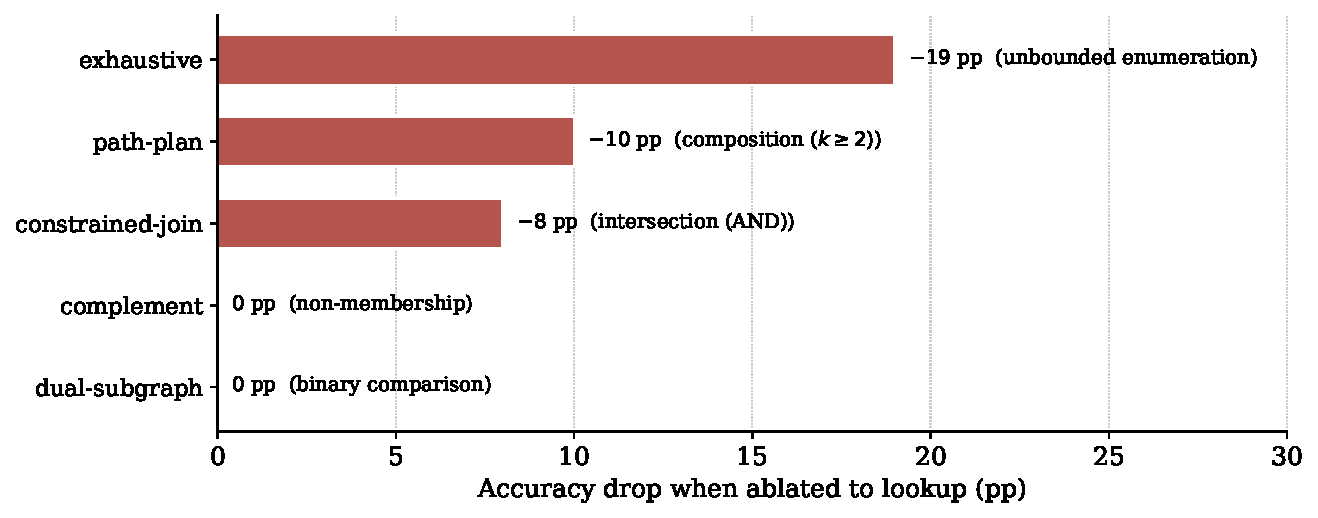
\includegraphics[width=0.92\linewidth]{figures/fig3_ablation.pdf}
\caption{逐算子消融:将每个算子回退为 \op{lookup} 时的准确率下降。三个承重算子针对互不相交的答案几何类别;\op{complement} 与 \op{dual-subgraph} 在本基准的"否定/比较"分布上读数为 0 个百分点,源于分布而非冗余。}
\label{fig:ablation}
\end{figure}

\subsection{增益来自何处}
一次预言机分发器消融(用金标问题类型路由)达到 88.2\%——与 LLM 分发(88.6\%)相差仅 0.4 个百分点——因此全部增益是\emph{算子驱动}的,而非分类器侥幸。逐算子消融显示三个承重算子作用于互不相交的题目切片(图~\ref{fig:ablation}):去掉 \op{exhaustive} 损失 $-19$ 个百分点、\op{path-plan} $-10$、\op{constrained-join} $-8$(合计 $-37$ 个百分点,占据可恢复的失败预算)。为排除"基线太弱"的伪命题,我们在两个 7B 底座(含 RoG 原始底座)上 LoRA 微调路径规划器,各自较其零样本版本提升约 $+30$ 个百分点,但仍落后 Strategy $+27$ 至 $+33$ 个百分点:单路径规划器无法表达集合代数算子。

\subsection{多步智能体质量、成本与迁移}
在一个 72 任务的组合套件(六类算子组合,金标由确定性执行器给出)上,智能体达到 100\% 有效计划、100\% 可执行、99\% 答案正确——诚实的告诫是:这衡量的是规划器质量(以确定性真值执行器为基准、模板生成的任务)。端到端成本为 \textbf{\$0.00041 每查询}(每准确率点 \$0.00084),完全落在面向分析员工具的可部署预算之内。最后,类型学与分发器可零重训迁移到 \textbf{KQA Pro} \citep{cao2022kqapro}(Wikidata)(67.4\% 零样本路由匹配;\op{dual-subgraph} 在 SelectBetween 上 $+11$ 个百分点),表明该引擎并非对雷达领域过拟合。作为完全外部的结构性检验,我们还构建了一张 19\,540 条三元组的 Wikidata 图谱(影视域)、金标经 SPARQL 计算——KB 与金标均非我们编写——并生成 157 道镜像答案几何类型的题目。在高基数类型上(金标中位基数 117),被宽松地预言机抽取的 top-$K{=}20$ 基线只召回 0--4\%,而类型化算子召回 100\%,single-hop 对照打平于 100\%:结构性增益在独立 KB 与金标上重现(确定性、算子级测试)。

\subsection{对抗决策支持:条令保真性与溯源}
\label{sec:eval-ew}
对抗模块在两条对决策支持工具至关重要的维度上评估:建议是否符合条令,以及每条结论是否可审计?

\paragraph{条令保真性。} 在 16 个取自电子战教科书的手工策展案例上——\emph{独立}真值,而非引擎自身规则——推荐器在 \textbf{16/16} 个案例中均"包含正确的条令技术且排除错误技术"(例如单脉冲火控 $\to$ 交叉眼/交叉极化,\emph{而非}倒相增益;频率捷变搜索 $\to$ 拦阻/扫频,\emph{而非}瞄准式噪声)。在全部 \textbf{650} 份威胁画像上,引擎不变量无一例外成立(\textbf{0} 违例):被推荐的技术绝不同时被列为应避免或被抵消,所引条令规则均可解析,且推荐装备的频段始终与威胁匹配。支撑这些建议的知识库覆盖 \textbf{89} 部 SAM/IADS 威胁雷达与 \textbf{4} 个有据可查的历史 SEAD 交战案例(Fan Song、Straight Flush、Low Blow、Flat Face),用作独立的合理性校验。端到端地,一个由五部辐射源组成的 S-400 防空群可由一个两件套装备包覆盖(5/5 加权威胁),且正确识别出 SEAD 优先目标(92N6 交战雷达)。

\paragraph{溯源/可审计性。} 由于事实绝不源自 LLM,可审计性是可度量而非空口断言的。在 30 份抽样情报档案上,\textbf{100\%} 的确定性事实(458/458)都携带来源与置信度,且 LLM 执行摘要 \textbf{100\%} 接地:摘要中的每个实体与数字记号都可追溯到一条被引用的事实,\textbf{30/30} 份报告零臆造。这把 \S\ref{sec:agent} 的"LLM 不进入信任路径"设计加以量化。

% =========================================================================
\section{部署考量、可信度与局限}
\label{sec:deploy}

\paragraph{可信度与失败代价。}
由于事实与数字仅来自确定性算子,分析员需提防的失败模式是有界且可读的:图谱中缺失的边(以低覆盖率 $N/M$ 暴露,绝不被悄悄补全)、超出覆盖的型号(以"未收录"暴露,并转入一次被标记为未核验、置信 0.6 的联网查询)、或分发器误路由(其会优雅降级为混合 \op{lookup},而非退化为某个错误算子的空集)。没有任何失败模式能让 LLM 把臆造参数写进报告。

\paragraph{局限。}
本系统是一套方法论与研究级试验台,而非一个经认证的作战工具:知识图谱由开源与公有领域来源构建,故对任一真实威胁的绝对覆盖受限于数据获取,而非方法本身。基准对照执行器自动生成,因此衡量的是结构正确性而非分析员判定的有用性;人在回路研究属未来工作。六类信息需求虽有依据,却未被证明完备——聚合算术、传递闭包与时间区间约束都将催生更多算子。

% =========================================================================
\section{相关工作}
\label{sec:related}

\textbf{知识图谱问答与 GraphRAG。} 综述 \citep{peng2025graphrag} 与系统 \citep{edge2024graphrag,gutierrez2024hipporag} 把 LLM 接地于图谱;推理路径方法 \citep{luo2024rog,sun2024tog,ma2025tog2,jiang2023structgpt} 与 KG 增强提示 \citep{baek2023kaping} 都检索一个按相关性排序的 top-$K$ 集合。\textbf{自适应检索。} Adaptive-RAG \citep{jeong2024adaptiverag} 按查询\emph{复杂度}路由,ByoKG-RAG \citep{byokgrag2025} 融合多种 KG 检索工具,但二者都保持检索原语不变;我们则改变原语的\emph{语义}(求交 vs 枚举 vs 求补 vs 组合)。\textbf{认知电子战决策支持。} 雷达干扰决策 \citep{zhang2023cognitiveew} 与经典电子战条令 \citep{adamy2001ew101,schleher1999ew} 启发了对抗模块;我们的贡献在于通过把建议接地于一个带溯源的知识图谱并用集合覆盖形式化 \citep{chvatal1979setcover},使该建议\emph{可审计}。

% =========================================================================
\section{结论}
\label{sec:conclusion}

我们提出了一个面向雷达电子战情报分析的、智能且可审计的决策支持系统。其核心洞见——top-$K$ 检索隐含了一个在分析员最棘手问题上失效的答案几何假设——催生了一套类型化算子族,把决策质量从 52.7\% 提升到 88.6\%,同时使语言模型不进入信任路径,因此每条结论与每条对抗建议都可追溯到来源。系统单次查询成本 \$0.00041 即可部署,其引擎可迁移至雷达领域之外。我们公开发布基准与知识图谱,以支持"让检索匹配决策真正所需答案之几何"这一方向上的可复现研究。

% =========================================================================
\section*{CRediT 作者贡献声明}
\textbf{作者姓名:} 概念化、方法学、软件、数据策展、形式化分析、验证、可视化、初稿撰写、审阅与编辑。

\section*{利益冲突声明}
作者声明不存在任何可能影响本文所报告工作的已知竞争性经济利益或个人关系。

\section*{数据可得性}
RadarKG-QA-499 基准、RadarKG-v2 知识图谱以及评估与系统代码已公开于 \url{https://github.com/syx7597/radarkg-qa},并将在录用后归档并赋予永久 DOI。

\section*{资助}
本研究未获得公共、商业或非营利部门资助机构的任何专项资助。

\section*{科研写作过程中的生成式 AI}
大语言模型是所提系统的一个功能组件(分发器、规划器与作答措辞阶段),如文中所述。此外,在稿件准备过程中作者仅使用 AI 助手进行语言润色;全部科学内容均由作者审阅与核验,作者对本出版物承担全部责任。

\bibliographystyle{unsrtnat}
\bibliography{references}

\end{document}
